%
% This template has been downloaded from:
% http://www.LaTeXTemplates.com
%
% Original author:
% WikiBooks (http://en.wikibooks.org/wiki/LaTeX/Title_Creation)
%
% License:
% CC BY-NC-SA 3.0 (http://creativecommons.org/licenses/by-nc-sa/3.0/)
%
% TRADUZIDO POR REBECA BACANI
%
%%%%%%%%%%%%%%%%%%%%%%%%%%%%%%%%%%%%%%%%%
% ----------------------------------------------------------------------------------------
%	PACKAGES AND OTHER DOCUMENT CONFIGURATIONS
% ----------------------------------------------------------------------------------------

\documentclass[12pt]{article}
% \usepackage[english]{babel}
\usepackage[portuguese]{babel}
% \usepackage[T1]{fontenc}
\usepackage[utf8x]{inputenc}
\usepackage{amsmath}
\usepackage{graphicx}
\usepackage[colorinlistoftodos]{todonotes}
\usepackage{indentfirst}		% Indenta o primeiro parágrafo de cada seção.
\usepackage{lipsum} %pacote para geração de texto de mentirinha
\usepackage{float} %pacote para mandar nas figuras!
\usepackage[version=3]{mhchem} % Formulas químicas usando \ce{} exemplo \ce{CH4} vai fazer o 4 subscrito direto.
\usepackage{dcolumn,bm,verbatim,cprotect,url,color,caption}
\usepackage{hyperref}

%% Determinação das cores de hyper-referência.
\hypersetup{
  colorlinks=true,
  citecolor= violet,
  linkcolor=blue!85,
  filecolor=magenta,
  urlcolor=cyan,
}


\usepackage[brazilian,hyperpageref]{backref}




% ProvidesClass{abntex2}
% \usepackage{abntex2abrev}
% \usepackage[alf]{abntex2cite}	% Citações padrão ABNT
\usepackage{csquotes}
\usepackage{titlesec}
\setcounter{tocdepth}{4}
\setcounter{secnumdepth}{4}
\graphicspath{{./images/}}
\usepackage{breakcites}


\newlength{\ABNTEXcitacaorecuo}% recuo de 4 cm da margem esquerda
\setlength{\ABNTEXcitacaorecuo}{4cm}
\newcommand{\ABNTEXfontereduzida}{\footnotesize}

% \usepackage[singlespace]{setspace} % para fazer com que SingleSpace funcione

\newenvironment*{citacao}[1][default]{%
  \list{}%
  \ABNTEXfontereduzida%
  \addtolength{\leftskip}{\ABNTEXcitacaorecuo}%
\item[]%
  % \begin{SingleSpace}%
  \ifthenelse{\not\equal{#1}{default}}{\itshape\selectlanguage{#1}}{}%
  % {%
  % \end{SingleSpace}%
  \endlist}%


\usepackage{nomencl} %% Lista de siglas
\makenomenclature    %% Fazer lista de nomeclaturas
\renewcommand{\nomname}{\listadesiglasname}

% ---

\begin{document}

\begin{titlepage}

  \newcommand{\HRule}{\rule{\linewidth}{0.5mm}} % Defines a new command for the horizontal lines, change thickness here

  \center % Center everything on the page

  % ----------------------------------------------------------------------------------------
  %	HEADING SECTIONS//// CAPA!
  % ----------------------------------------------------------------------------------------

  \textsc{\LARGE Universidade de São Paulo}\\[1cm] % Name of your university/college
  \textsc{\Large Escola de Engenharia de Lorena}\\[0.5cm] % Major heading such as course name
  % \textsc{\large Minor Heading}\\[0.5cm] % Minor heading such as course title

  % ----------------------------------------------------------------------------------------
  %	TITLE SECTION//// Título
  % ----------------------------------------------------------------------------------------

  \HRule \\[0.4cm]
  {\huge \bfseries Fora do imaginário comum: \textit{software} livres, impactos na política, economia, e academia\\[0.4cm] LOM3243-Seminários em EF}\\[0.4cm]
  \HRule \\[1.2cm]
  % Substitua esse treço pelo seu título

  % ----------------------------------------------------------------------------------------
  %	AUTHOR SECTION//// Autor
  % ----------------------------------------------------------------------------------------

  % \begin{minipage}{0.4\textwidth}
  %   \begin{flushleft} \large
  %     \emph{Aluno:}\\
  %     Max von Laue\\  %Nome do aluno
  %   \end{flushleft}
  % \end{minipage}
  ~
  \begin{minipage}{0.4\textwidth}
    \begin{center} \large
      \emph{Grupo} \\
      Aexandre H. C. Leal \\%colaboradores aqui!
      Camila O. Cardoso \\
      Pedro G. Branquinho \\
      Igor H. C. Yamamoto \\
      Henrique S. Julio \\
    \end{center}
  \end{minipage}\\[0.8cm]

%%%%%%%%%%%%%%%%%%%%%%%%%%%%%%%%%%%%%%%%%
  % ----------------------------------------------------------------------------------------
  %	LOGO SECTION/// Logo USP
  % ----------------------------------------------------------------------------------------

  
\includegraphics[width=3cm]{logo.png}\\[2cm] % já colocado

  % ----------------------------------------------------------------------------------------
  %	DATE SECTION/// Data
  % ----------------------------------------------------------------------------------------

  {\today}\\[0.5cm] % Date, change the \today to a set date if you want to be precise


  % ----------------------------------------------------------------------------------------

  \vfill % Preenche o resto da página com espaços em branco

\end{titlepage}



\pdfbookmark[0]{\listfigurename}{lof}
\listoffigures
\cleardoublepage

{\flushleft{\Large{\textbf{{\scshape{Lista de Nomeclaturas}}}}}}
\nomenclature{SL}{Software Livre}
\nomenclature{NM}{nomeclatura}
\nomenclature{GNU}{GNU's Not Unix}
\nomenclature{CISL}{Comitê Técnico para Implementação do Software Livre}
\nomenclature{ITI}{Instituto Nacional de Tecnologia da Informação}
\nomenclature{PSL}{Portal Software Livre}
\nomenclature{ePING}{Padrões de Interoperabilidade de Governo Eletrônico}
\nomenclature{Embrapa}{Empresa Brasileira de Pesquisa Agropecuária}
\nomenclature{SPB}{Portal do Software Público Brasileiro}
\nomenclature{ODF}{Open Document Format}
\nomenclature{XML}{eXtensible Markup Language}
\nomenclature{ISP}{Internet Service Provider}
\nomenclature{SERPRO}{Serviço Federal de Processamento de Dados}
\nomenclature{OS}{Open-Source}
\nomenclature{OSI}{Open-Source Initiative}
\nomenclature{SERPRO}{Serviço Federal de Processamento de Dados}
\nomenclature{CACIC}{Configurador Automático e Coletor de Informações}





\pdfbookmark[0]{\nomname}{las}
\printnomenclature
\cleardoublepage


\pdfbookmark[0]{\contentsname}{toc}
\tableofcontents
\cleardoublepage






% ----------------------------------------------------------------------------------------
%	TEXT/// Início do texto
% ----------------------------------------------------------------------------------------
\begin{abstract}
  A diferenças práticas e filosóficas entre
  \textit{softwares} proprietários e livres. Entendê-los, em nosso contexto
  histórico, é parte da cidadania. O movimento
  do software livre começa na década de oitenta, no ambiente
  universitário do MIT, e repercute-se aos dias atuais, por meio da
  perpetuação de estruturas as quais prezam pelos direitos dos
  usuários, garantindo-lhes a liberdade de estudar, modificar e compartilhar os \textit{softwares} os
  quais operam grandes porções de suas vidas
  virtuais. Estudaremos as
  implicações cibernéticas dos \textit{softwares} livres em quatro esferas,
  filosófica-conceitual, mercadológica, acadêmica e
  governamental. A pesquisa é uma revisão
  bibliográfica. Procuramos, na literatura, a interação do software
  livre com essas quatro esferas. Há uma falta de estudos sistematizados sobre os
  impactos dos \textit{softwares} livres. É
  possível observar diversas vantagens em se utilizar o software
  livre, porém, ainda existem sólidas barreiras culturais ao seu
  uso. Há uma necessidade de maior integração
  prático-teórica na sociocultural da nossa sociedade, para a adoção
  efetiva do software livre e suas implicações.

\end{abstract}

\newpage

\section{Introdução}

\label{cap: intro}
A tecnologia avançou e sofreu inúmeras mudanças nas últimas décadas. Desde aplicações de estruturas na escala quântica para impulsionar o nível de processamento de computadores até a manifestação de oscilações gravitacionais advindas da interação de buracos negros localizados a anos-luz de distância da Terra. De fato, o estado atual científico se semelha à um filme \textit{sci-fi}, onde os mais inesperados utensílios surgem, com precisões e eficiências nunca vista antes.

Porém, quando se trata de senso comum, a palavra ``tecnologia'' automaticamente remete a um tópico principal: internet e computação. O rápido desenvolvimento de novos modelos de dispositivos microeletrônicos, a otimização dos meios de transmissão de dados, em conjunto ao grande potencial da ciência de dados, proporcionaram a possibilidade de serem criadas diversas tecnologias cibernéticas que atualmente não só dominam o mercado econômico, mas que também estão presentes na vida de qualquer indivíduo da nossa sociedade. De acordo com a União Internacional de Telecomunicações, em 2019, 4,1 bilhões de pessoas tinham acesso à rede, referente a 53,6\% da população mundial \cite{onu2019}. Já no Brasil, o IBGE constatou que, em 2017, 74,9\% dos domicílios tinham acesso à Internet, sendo a sua grande maioria concentrada em centros urbanos \cite{ibge2017}.

Para muitos, porém, os celulares e computadores são nada além de mágicas ``caixas-pretas'', que interpretam e respondem a comandos específicos. Uma ínfima parcela da população de internautas possuem conhecimentos sobre alguns dos tópicos básicos de computação, como linguagens de programação, protocolos, arquitetura e componentes eletrônicos. Muito menos ainda conhecem aspectos que circundam esta tecnologia, como questões jurídicas, implicações econômicas e socioculturais, e até mesmo bases filosóficas e conceituais que fundamentam e direcionam como uma rede ou um \textit{software} deve ser projetado.

Este texto tem apenas um objetivo: introduzir o conceito de \textit{Open-Source} (OS), uma ideia que surgiu nos meados de 1980 e então amadurecida por alguns cientistas da computação, cujo objetivo é fazer com que códigos computacionais referentes à um dado projeto sejam libertos por completo junto ao \textit{software}. Apontaremos, assim, ao impacto que este ideal possui sobre todas as tecnologias de informação que estão presentes no mercado atual, e como ele mudou, continua a mudar e promete mudanças sobre as nossas estruturas de relação sociais, econômicas e culturais.

\newpage

\section{Revisão Bibliográfica}
\subsection{Conceitos e filosofia}
O modelo de negócio empregado pela esmagadora maioria das empresas detentoras de patentes se constitui em produzir e vender em larga escala os seus produtos, acompanhados de informações obrigatórias de serem compartilhadas e que são particulares do tipo do produto. Por exemplo, a Agência Nacional de Vigilância Sanitária (ANVISA) obriga que alimentos comercializados apresentem um rótulo nutritivo, contendo uma série de informações acerca da composição do produto e que, caso não fosse compartilhado, poderia ser nocivo à saúde de um determinado nicho de consumidor \cite{anvisa}. Porém, ela não obriga que o fabricante compartilhe também a ``receita'' utilizada para a confecção, respeitando os seus direitos autorais e intelectuais.

Assim como mencionado, esta dinâmica se repete em outros segmentos, incluindo o mercado de computação. A Microsoft, ao realizar a venda de seus produtos, como por exemplo o sistema operacional Windows ou o pacote Office, entrega ao consumidor um compilado de arquivos em  binários (ou seja, escritos em linguagens de máquinas, e que podem ser apenas interpretados por máquinas), que por sua vez são de difícil acesso e inviáveis de serem realizadas modificações. Esta técnica de distribuição e venda de arquivos executáveis é empregada também por outras gigantes do segmento tecnológico, como a Apple Inc., Adobe Systems Inc., Oracle, dentre muitas outras \cite{wiki_prop_source2020}.

Porém, é importante notar que cada segmento industrial e tecnológico possui as suas singularidades, e isso diz respeito também à forma que é feita a distribuição de seus produtos. De fato, não temos um sistema político, econômico e social que se ampara nas limitações que são impostas pelas receitas secretas da Coca-Cola, o que não é verdade quando se trata de computadores e \textit{softwares}: todas as relações na era de dados são impactadas pela funcionalidade e, principalmente, pela portabilidade das ferramentas computacionais que são desenvolvidas e utilizadas. Restringir o público a usar um \textit{software} de uma forma particular constringe as possibilidades de inovação e acumula as responsabilidades de conserto de \textit{bugs} apenas à empresa detentora dos direitos autorais da ``receita'' do programa. O consumidor, assim, fica à mercê da empresa, e nenhum direto lhe é assegurado caso deseje experimentar de novas funcionalidades ou realizar mudanças particulares.

O problema de constrição possui uma saída simples: compartilhar, junto ao produto, o código fonte que gera os arquivos em linguagem de máquina - ou seja, compartilhar a ``receita''. E é nisso que se baseia o conceito de OS (código aberto). Aqui, os usuários não apenas adquirem o \textit{software}, mas também são assegurados do direito de, caso desejem, poder realizar mudanças e também a distribuição. Uma definição mais formal pode ser encontrada no portal eletrônico da \textit{Open Source Initiative} (OSI) \cite{osi2020}, mas, resumidamente, pode ser definida por três fatores \cite{Weber2005}:
\begin{itemize}
\item O código fonte deve ser distribuído com o \textit{software} ou então ser disponibilizado por não mais que o custo de distribuição
\item Qualquer pessoa pode redistribuir o \textit{software} abertamente, sem \textit{royalties} ou taxas de licenciamento
\item Qualquer pessoa pode modificar o \textit{software} ou derivar dele outro software, e então distribui-lo sob os mesmos termos
\end{itemize}

Um erro conceitual cometido frequentemente sobre este conceito é associar ``\textit{open}'' com valores monetários. Parafraseando Richard Stallman \cite{gnu_what_is_open_source}:

\begin{displayquote}
  Por ``\textit{software} livre'' devemos entender aquele \textit{software} que respeita a liberdade e senso de comunidade dos usuários. Grosso modo, isso significa que os usuários possuem a liberdade de executar, copiar, distribuir, estudar, mudar e melhorar o software. Assim sendo, ``\textit{software} livre'' é uma questão de liberdade, não de preço. Para entender o conceito, pense em ``liberdade de expressão'', não em ``cerveja grátis''.
\end{displayquote}
A ideia de monetizar qualquer produto OS parece utópica em primeira instância. Porém, isso é verdade apenas sobre a luz do modelo de negócio já citado acima. Empiricamente, se nota que a economia de tecnologia de informação atual é dominada por códigos abertos: mais de 65\% dos servidores rodam a base de Apache, a maioria dos \textit{clusters} computacionais empregam Linux como o seu sistema operacional, e até mesmo governos estão iniciando atividades com códigos abertos \cite{Weber2005, wiki_usage_share}. Aos poucos, se nota que a liberdade e a robustez proporcionado por sistemas operacionais abertos está sendo adotado como opção de escolha por diversos segmentos não apenas da indústria, mas até mesmo para uso pessoal, dado a crescente comunidade de colaboradores presentes em fóruns como \textit{StackOverflow}.

\subsubsection{Richard Stallman e o projeto GNU}
Mas como que este movimento surgiu? A quem é atribuído a sua criação e como que um projeto tão ambicioso se tornou realidade?

A sua origem parte da insatisfação de alguns cientistas da computação que trabalhavam no laboratório de Inteligência Artificial do MIT (\textit{MIT AI Lab}) nas décadas de 70 e 80. O motivo da insatisfação? A substituição do sistema operacional \textit{Incompatible Timesharing System} (ITS), que era portável e compartilhável, pelo sistema proprietário pertencente à empresa Digital. A implicação imediata desta transação era a falta de portabilidade dos códigos desenvolvidos pelos pesquisadores, o que instaurava um sentimento de não-cooperação. Dentre eles se encontrava Richard Stallman, um estudante de PhD em Física, mas que se dedicava inteiramente à sua carreira de programador no \textit{MIT AI Lab}, e que foi um dos maiores expoentes no fomento do movimento OS. Notando a grande evasão de muitos pesquisadores do circuito dos \textit{hackers}, Stallman percebe que a tendência de imposições restritivas sobre os códigos aumenta, e que se nada fosse feito essa seria então a norma em poucos anos.

Assim, se demite de seu posto de pesquisador no laboratório de Inteligência Artificial para se dedicar a um único projeto: o desenvolvimento de um sistema operacional aberto. Este sistema deveria ser aberto a fim de se permitir a cooperação de outros hackers da comunidade. Ainda, ele seria compatível com o sistema Unix (pertencente, até então, à empresa AT\&T), visando portabilidade e a facilidade de migração de novos usuários. O nome escolhido para este novo sistema era GNU, que significava ``GNU is Not Unix'', ironicamente um acrônimo recursivo que usa o próprio nome para se definir \cite{wiki_gnu, Stallman_gnu2019}.

O desenvolvimento deste projeto demandava não apenas o sistema operacional em si, mas também de outros programas e estruturas, como processadores de comando, compiladores, interpretadores, depuradores e editores de texto, assim como era presente nos demais sistemas. Para executar tamanho projeto, então, Stallman decidiu por redigir um manifesto, chamado de ``O Manifesto GNU'' \cite{Stallman_manifesto2019}, para tanto pedir apoio no desenvolvimento de seu projeto quanto alinhar os futuros desenvolvedores de quais eram os principais princípios envolvidos. Mais tarde, com o desenvolvimento do núcleo computacional (``\textit{kernel}'') Linux, escrito por Linus Torvalds, o sistema GNU e o \textit{kernel} foram combinados, a fim de se formar um sistema operacional livre e completo, intitulado ``GNU/Linux'' \cite{Stallman_gnulinux2019} (este que é comum e erroneamente chamado apenas por ``Linux'').

\paragraph{Licenças e o GNU GPL}
Para que o projeto fosse distribuído de acordo com os seus objetivos de liberdade e distribuição, foi necessário implementar um método jurídico que possibilitasse e assegurasse os usuários de seus direitos. Este método é chamado de \textit{Copyleft}: basicamente a inversão dos \textit{Copyright}, ou seja, tem como objetivo retirar as barreiras ao uso, difusão e modificação de uma obra criativa, exigindo ainda que o mesmo seja aplicável em versões modificadas \cite{wiki_copyleft}. A implementação específica deste método foi através da Licença Pública Geral GNU (\textit{GNU General Public License}). Nela, todos os \textit{softwares} distribuídos tinham assegurados os direitos mencionados no manifesto \cite{Brett2019}. Ainda, outras licenças foram também criadas para servir outros objetivos, como, por exemplo, a Licença Pública Geral Menor GNU (\textit{GNU Lesser General Public License}, ou GNU LGPL, que servia o objetivo de proteger bibliotecas) e a Licença de Documentação Livre GNU (\textit{GNU Free Documentation License}, garantindo que qualquer um tenha a liberdade de usar e redistribuir manuais, livros e documentos).

Ao longo do tempo outras licenças OS surgiram, apresentando nuanças diferenciadas da licença GPL. Algumas delas são: \textit{MIT License} \cite{mit_license}, \textit{Apache License} \cite{Apache_license} e \textit{BSD License} \cite{bsd_license}. É importante notar que reformulações nos termos são feitas através da atualização de versões de licenças. Atualmente, a licença mais utilizada é a MIT, seguida da Apache 2.0 e então da GPL 3.0 \cite{os_trend}.

\subsubsection{Relevância da filosofia OS}
É indiscutível a relevância do paradigma de livre distribuição de código na tecnologia. Ela impulsionou drasticamente a dinâmica de criação de novas ferramentas, e códigos abertos são utilizados e criados constantemente por ``\textit{tech giants}'', como o Google, Facebook, Amazon, Yahoo, dentre muitas outras.

A ideia por trás deste movimento ainda trouxe questionamentos acerca de possíveis mudanças estruturais na nossa sociedade que poderiam ser melhoradas. Segundo Steven Weber \cite{Weber2005}:

\begin{displayquote}
  As pessoas normalmente veem no movimento OS a política que eles gostariam de viver - uma perfeita meritocracia, um presente cultural utópico, que celebra uma economia de abundância ao invés de escassez, uma prova virtual ou eletrônica de ideais comunitários, um movimento político focado em substituir as estruturas obsoletas do capitalismo com novas relações de produção, mais adaptadas à era da informação.
\end{displayquote}

Dentre uma das maiores lições deste movimento, encontra-se a colaboração. Desde ferramentas de gestão de projeto focadas na imersão e responsabilidade de todos os membros do grupo, como o SCRUM e Agile, até novas abordagens para fomentar a inovação, como o Design Thinking, exigem ambientes onde a colaboração é crucial para se adaptar ao novo modelo de mercado. Esta noção de colaboração, derivada do OS, se estende atualmente a diversos segmentos da indústria, não estando mais apenas limitado ao mercado de desenvolvimento de software \cite{raconteur}.

Hoje em dia também diversos especialistas estudam a possibilidade de implementar a filosofia e os métodos jurídicos derivados do OS à outros domínios. Em contraste ao movimento código aberto, existe também atualmente o chamado ``Hardware aberto'', o qual busca abrir a possibilidade de estudo, modificação, criação e distribuição para o desenvolvimento de objetos físicos de forma livre e licenciada \cite{open_hardware}.

Um extremo desta abordagem é visionar não apenas ferramentas tecnológicas como podendo ser abertas, mas sim qualquer tipo de informação. Em seu livre ``\textit{The Open Revolution}'' \cite{Pollock_2018}, o autor Rufus Pollock propõe que a economia digital ``fechada'' é a fonte de diversos problemas, como acumulo de poder de monopólios tecnológicos, a crescente desigualdade mundial, o alto custo de medicamentos e até mesmo a forma que a população pensa e vota. Ele afirma que, no futuro, a opção adotada pela grande massa será de realizar e aceitar os métodos de distribuição similares aos utilizados para os códigos abertos, e isso se estenderia à todos tipos de dados digitais, como educação, ciência, artes e notícias.


\subsection{Aplicação nas empresas}

\subsubsection{\textit{Softwares} livres e o mundo empresarial}

O \textit{software} livre está cada vez mais presente na atuação das empresas do mundo, empresas como IBM, Amazon, Google e Intel já utilizam \textit{softwares} livres como Linux, Apache, PHP, MySQL, Sendmail e Open Office, dentro de seus processos. Além disso, tais empresas utilizam dos \textit{softwares} livres para a disponibilização de alguns de seus recursos \cite{cerqueira2011}. Graças a uma pesquisa em conjunto com a Unicamp e o ministério da Ciência e da Tecnologia, constatou-se que no Brasil há uma divisão das empresas em três grupos distintos quando se trata de \textit{software} livre, o primeiro são pequenas e médias empresas, fundadas entre 1980 e 1990, que fazem uso majoritariamente de \textit{softwares} proprietários, o segundo são pequenas e médias empresas mais recentes que surgiram devido aos \textit{softwares} livres e que possuem grande parte de suas atividades utilizando \textit{softwares} livres, por fim existem as grandes empresas que cada vez mais estão utilizando de \textit{softwares} livres dentro de seus processos de forma estratégica para obter alguns benefícios que estes podem oferecer \cite{cerqueira2011}, SOFTEX;UNICAMP, 2005].

A pesquisa também mostrou algumas estatísticas interessantes quanto a utilização dos \textit{softwares} livres dentro das empresas brasileiras. O \textit{software} Linux é o segundo mais utilizado nas empresas com um geral, sendo utilizado em 56\% dos servidores das médias empresas e em 53\% dos servidores das grandes empresas. Tal estatística mostra a rivalidade desse \textit{software} com o Unix, utilizado nas grandes empresas, e do Windows que atualmente é o mais utilizado em geral devido a sua facilidade de interação com usuário que não possuem tanto conhecimento de computação \cite{cerqueira2011}, apud SOFTEX;UNICAMP, 2005].

Para somar com as estatísticas, uma pesquisa realizada pelo ISF (Instituto Sem Fronteiras) registrou que 73\% de empresas com mais de mil funcionários utilizavam \textit{softwares} livres, enquanto apenas 31\% das empresas com até 99 funcionários utilizavam \textit{softwares} livres em alguma atividade \cite{serpro2008}. Dessa forma é possível notar que as empresas de médio e grande porte tem uma preferência maior no uso de \textit{softwares} livres do que as empresas de pequeno porte, algo que vai contra o senso comum.

Uma multa No Brasil pode chegar a até 3 mil vezes o valor do \textit{software}, isso tornaria a “economia” de utilizar o \textit{software} proprietário pirateado em uma enorme perda \cite{serpro2008}.  No entanto, a supervisão desse tipo de infração é quase que inexistente para pequenas empresas no país, sendo apenas feita apenas para médias ou grandes empresas, esse fenômeno influência no comportamento das pequenas empresas de evitar o uso de \textit{softwares} livres para redução de custo, pois podem utilizar de forma ilegal, e sem serem multadas, \textit{softwares} proprietários [Reis, 2008, apud SILVA,2006].

\subsubsection{Uso comercial dos \textit{softwares} livres dentro das empresas}

Como foi escrito acima, muitas empresas utilizam o \textit{softwares} livres em seus servidores e algumas até em computadores dos usuários, como por exemplo a Google e a Amazon que utilizam Linux nos computadores de todos os seus desenvolvedores.  No entanto, o principal ramo comercial dos \textit{softwares} livres está na área de prestação de serviços para obtenção de receitas. Tais serviços podem ser alterar programas para resolver problemas específicos, melhorar programas ou prestar consultoria e treinamentos para outras empresas que estão se adaptando ao uso de \textit{software} dentro da sua dinâmica de atividades, dessa maneira as receitas vem da venda do serviço e não do software em si \cite{saleh2004}.

Basta pensar em uma grande empresa, ou média empresa que deseja alterar as suas ferramentas para aderir ao uso de \textit{softwares} livres, para isso ela precisará capacitar sua equipe e precisará instalar corretamente todos os \textit{softwares}, nesse momento uma terceira, já capacitada e com gente treinada irá auxiliar nessa transição, treinando e preparando o novo ambiente de trabalho da empresa, por esse serviço prestado que a terceira irá obter receitas utilizando do \textit{software} livre. Algumas empresas, como a Embrapa, visualizando essa transição de \textit{softwares} proprietários para livres, criaram um setor focado no desenvolvimento e aplicação de \textit{softwares} livres \cite{embrapa2020}.

\subsubsection{Vantagens e desvantagens do uso de \textit{softwares} livres }

O uso dos \textit{softwares} livres traz uma série de benefícios para as empresas, principalmente as de médio e grande porte que possuem servidores e muitas máquinas. Um benefício imediato é a redução dos custos que empresa precisará despender com as licenças dos \textit{softwares} proprietários que precisariam ser pagar periodicamente e por número de máquinas \cite{sebrae2020}. Assim, empresas que possuem bastantes computadores não precisará desembolsar uma quantia maior do que uma empresa com menos computadores, pois não precisará pagar licenças para o uso ou pelo número de máquinas utilizando o \textit{software}, tornando tais empresas mais competitivas no mercado.

Os \textit{softwares} livres ajudam no combate ao aprisionamento tecnológico devido a liberdade que ele possui em sua licença \cite{saleh2004}, a própria definição de \textit{software} livre implica na liberdade para reprodutibilidade e adaptabilidade do \textit{software}. Dessa maneira as empresas podem modificar tais \textit{softwares} para que eles atendam de forma mais específica as suas necessidades.

Além desses dois fatores, os \textit{softwares} livres contribuem para uma redução nas despesas em relação aos \textit{hardwares} \cite{saleh2004}. Os \textit{softwares} livres possuem um ótimo desempenho em equipamentos mais antigos, o que permite um maior tempo de vida útil para tais equipamentos, permitindo um maior tempo entre as trocas dos aparelhos \cite{Gusman2002}, permitindo assim uma economia no custo da troca de \textit{hardwares}.

Outra vantagem dos \textit{softwares} livres é garantia contra a descontinuidade do \textit{software}. Se uma empresa é proprietária de um \textit{software} qualquer, ela pode a qualquer momento fazer o que bem entender com a sua propriedade, desde alterá-lo ou até mesmo descontinuá-lo caso ela queira. Já um \textit{software} livre possui uma comunidade de programadores voluntários que se renova constantemente e que também utiliza daqueles recursos, dessa forma há uma segurança bem maior no quesito de atualização do \textit{software} devido a essa comunidade que tanto desenvolve quanto utiliza o \textit{software} \cite{saleh2004}.

Dessa maneira, caso um projeto de \textit{software} livre seja grande o suficiente, como no caso do Linux (\textit{software} livre de um sistema operacional que rivaliza com o Windows) o \textit{software} pode apresentar maior segurança, estabilidade, desempenho e qualidade do que o seu rival pago, devido à sua grande comunidade de programadores e usuários que periodicamente atualizam o \textit{software} melhorando-o constantemente [Saleh, 2004, apud Raymond, 2003].


Contudo, a adaptação do uso de ferramentas e novas metodologia de trabalho gera custos devido à iniciais perdas de produtividade e gastos com treinamentos da equipe, esses custos podem ser vistos como uma desvantagem pois serão necessários para que uma empresa que utiliza \textit{softwares} proprietários passe a utilizar \textit{softwares} livres \cite{cerqueira2011}.

\subsubsection {Problemas para a migração do sistema}

Como descrito no último parágrafo, um dos maiores problemas para o uso dos \textit{softwares} livres nas empresas é a migração do ambiente do \textit{software} proprietário utilizado para o ambiente \textit{software} livre. As principais adversidades dessa transição são o custo da migração, o tempo de migração envolvido e os problemas técnicos que podem ser gerados durante a migração. Além desses, existem outras barreiras para a disseminação do uso dos \textit{softwares} livres nas empresas como o desconhecimento, por parte das empresas, dos \textit{softwares} livres que poderiam substituir os \textit{softwares} proprietários utilizados \cite{saleh2004}.

Um fator interessante a se ressaltar em relação ao tempo de migração, é que o número da quantidade de dados que precisarão ser migrados de um \textit{software} para outro só tende a aumentar com o tempo o que facilita o aprisionamento tecnológico de uma empresa por conta da sua dificuldade em transferir os dados de uma plataforma para a outra e que com o passar do tempo acabam sendo reféns de um \textit{software} proprietário \cite{bilich2002}.


\subsubsection {Exemplos utilizados nas empresas}

Alguns exemplos de \textit{softwares} livres utilizados dentro das empresas estão relacionados a seguir com os seus similares proprietários.

Uso empresarial para as atividades do dia a dia de escritório, \textit{softwares} para produção de textos, planilhas e apresentações:

• OppenOffice, Koffice, Gnome Office x Microsoft Office (proprietário)

Uso para banco de dados:

• MySQL e PostgreSQL x AWS Amazon, Azure Microsoft, IBM Cloud

Uso para sistemas operacionais:

• Linux x Windows e Unix (proprietários)

Uso para gerenciamento de e-mails:

• Sendemail, Qmail x Outlook (obtido ao se pagar o Office 365)













\subsection{Aplicação na Academia}

\subsubsection{Definição de Software Livre}

Na definição do termo ``\textit{free software}'', estão listados três pontos
definitivos para o termo, chamada as quatro liberdades essenciais ``\textbf{A liberdade de estudar como o programa funciona, e
  modificá-lo para que ele opere como deseja.} Acesso ao código é uma pré-condição para essa liberdade.'' \cite{gnu_what_is_open_source},

% \begin{enumerate}
% \item A liberdade de rodar o programa com o usuário deseja, para
%   qualquer propósito.
% \item
% \item A liberdade de distribuir cópias gratuitas
% \item A liberdade de distribuir cópias gratuitas de versões modificadas.
% \end{enumerate}

% \subsubsection{Implicação da Definição à Aplicação Científica}

Dentro da segunda liberdade está explícita a ligação entre o software
livre e o método científico. Pois, para qualquer raciocínio em um
trabalho científico, deve-se ser explicado os passos para sua
conclusão. Desta forma, os leitores podem estudar, modificar e suplantar
aquelas ideias, hipóteses ou mesmo teorias. Por conseguinte, de forma
análoga, um software que segue as metodologias científicas quando
publicado, é, essencialmente, um \textit{software} livre.

\subsubsection{Cibernética e \textit{Software} Livre}
Dentro da perspectiva teórica da cibernética, em Sustentabilidade,
democracia e socio cibernética \cite{birrer1999}, parafraseia-se,

\begin{displayquote}
  A observação, o conhecimento e a análise se dão dentro da tentativa
  humana, contínua, de lidar e sintetizar experiências. E, apenas pode-se
  entendidas apropriadamente (as experiências) em um contexto orientativo, constituído
  pelas tentativas de resolução de um problema.
\end{displayquote}

Isto é, em nosso contexto, privar o acesso ao código fonte e à
extensão de um software é obstruir o progresso do conhecimento humano. Tornando-se, assim, um ato não só arbitrário, como
ideológico, com sérias implicações democráticas a longo prazo. Desta maneira, fica
clara a síntese da equipe GNU ``O programa não-livre controla o
usuário, e o desenvolvedor controla o programa; isso faz com que o
programa seja um instrumento que exerce poderes antidemocráticos.''  \cite{gnu1996}

\subsubsection{Graus de Liberdade Acadêmica}

Para a área acadêmica, também é possível observar a vasta diferença
entre as oportunidades de pesquisa, quando se utiliza um software
proprietário, em contrapartida ao software livre. Torna-se imposto ao
usuário do software proprietário não modificar a maneira com que as
operações são levadas.

Isto é, não há como modificar o comportamento
de um editor de texto, como o World. Não há opções de se estender uma
ferramenta de cálculos proprietário; caso não haver uma opção para se
calcular as derivadas ou integrais de uma função, não há a
oportunidade de implementá-las no código, pois roda-se em cima de
códigos binários. Há uma constrição desnecessária para o cientista.

\subsubsection{Comparação de Extensibilidade}

Quando se tem a opção de um software livre, ou um proprietário, a escolha em qualquer esfera deveria ser óbvia. O suporte da comunidade é outro
ponto essencial de divergência entre \textit{softwares} livres e proprietários. As comunidades livres são compostas de todos os
usuários-desenvolvedores do assunto. Assim, seu número é distantemente
maior à uma equipe de uma empresa a qual vende um software
velado.

Logicamente, nesse contexto, o suporte ofertado por uma empresa
seria diminuto em relação a sua opção livre, pelo número de
colaboradores técnicos, bem como a eventual capacidade de concertar
um problema específico incidental - visto que a modificação e personalização do software em
um contexto é proibida e indesejada, enquanto no outro é inerentemente aberta e
estimulada.


\subsection{Políticas governamentais e o \textit{software} livre}
O movimento do \textit{Software} Livre (SL) vem em contraponto à necessidade capitalista de adaptar às novas formas acumulação de bens, valorizando e precificando bens não materiais, fenômeno que começa a surgir em 1970 a 1980. Nesse cenário o SL vem para reivindicar que o conhecimento precisa ser livre e acessível às pessoas, não causando um aprisionamento tecnológico, e fazendo com que as pessoas fiquem livres da necessidade de licenças e limites no conhecimento da ferramenta que optam por utilizar. Desde então começa a haver uma articulação dos movimentos ligados ao SL na política, e que, no caso do Brasil, influenciaram a adoção de medidas favoráveis ao SL pelo governo brasileiro. \cite{torres2018software}.
\subsubsection{As diferenças entre o movimento \textit{free e open}}
Durante o desenvolvimento de toda teoria do \textit{Software} livre com Stallman, aconteceu o surgimento de outra vertente que defendia o emprego da nomenclatura "\textit{open source}" para tornar o produto e a ideia mais comercializável, seguindo objetivos neoliberais de gerar capital. Esse movimento entrou em oposição com as ideias de Stallman e principalmente com o seu discurso politizado, apoiado por um manifesto e a estruturação do que se chama de princípios éticos e as quatro liberdades que fundamentam o movimento \cite{evangelista2014movimento}.

Para uma breve contextualização histórica, o movimento do \textit{free software} ganha força e uma bandeira em 1983 com lançamento do projeto GNU por Richard Stallman. Já o movimento \textit{open source} ganha forma e força com Eric Raymond quando publica o artigo, em 1998, intitulado \textit{“Goodbye, ‘free software’; hello, ‘open source’”}, chamando a comunidade a deixar o termo \textit{free} e adotar o \textit{open}. No caso dos dois movimentos, esses eventos marcam quando eles ganham força e não quando nascem, pois já existiam ideias similares sendo articulados e pensados antes desses marcos acontecerem \cite{evangelista2014movimento}.

Com isso temos dois movimentos distintos que se separam filosoficamente em essência e dão origem a duas construções ideológicas distintas para se fazer o uso do \textit{software} livre, mas na forma prática de se adota-los, tratam de coisas muito similares\cite{torres2018software}.

\subsubsection{América latina, Brasil e o movimento político relacionado ao \textit{software} livre}
Afirma-se que a américa latina e inclusive o Brasil adotou a forma "\textit{Free Source}" de implantar essas tecnologias, também pensando na sua filosofia de acessibilidade de informação ao cidadão, e da posição política de se reafirmar contra a globalização corporativa e a aglutinação e prisão do conhecimento por grandes corporações\cite{torres2018software}.

Com relação ao uso político de \textit{Softwares} Livres, é possível apontar que os objetivos que fazem com que países como Brasil, Peru, Uruguai, Bolívia, Venezuela e Equador adotassem essa prática perpassam por alcançar uma vantagem econômica com relação a ausência de licenças pagas, mas também política na forma de valorizar a indústria nacional criando empregos localmente, desenvolvendo uma tecnologia nacional e escapar de práticas como espionagem feitas por meio dessas tecnologias importadas de grandes corporações que se alocam em países desenvolvidos. Essas pautas ascenderam e foram incorporadas na América Latina pela esquerda política, e com a ascensão de governos de esquerda no início dos anos 2000 \cite{torres2018software}.

\subsubsection{Políticas públicas acerca de software livre e seus resultados no Brasil }

O marco do Brasil na caminhada política da adoção nacional do \textit{Software} livre começou com o decreto de 29 de outubro de 2003. Esse decreto instituiu um comitê técnico que geriu a implementação do \textit{software} livre nos setores administrativos do governo e também projetos de inclusão digital\cite{torres2018software}.O principal comitê foi o intitulado Comitê Técnico para Implementação do \textit{Software} Livre(CISL), que traçava diretrizes para a incorporação dessas políticas, inclusive orientar, difundir e monitorar o cumprimento no governo federal, foi coordenado pelo Instituto Nacional de Tecnologia da Informação(ITI).Ainda em 2003 foi lançado o Portal \textit{Software} Livre(PSL) \cite{tiboni2014software}.

No final de 2004 ocorreu a consolidação da primeira versão dos  Padrões de Interoperabilidade de Governo Eletrônico(ePING), um documento em que se define um conjunto de regras e premissas que vão regulamentar a utilização da Tecnologia de Informação e Comunicação na interoperabilidade de Serviços de Governo Eletrônico. Esses parâmetros visam estabelecer as condições aceitas para a integração entre a esfera de serviços do governo federal e os demais poderes, e com sociedade em geral.

Em 2004, em conjunto com o ITI, a Empresa Brasileira de Pesquisa Agropecuária (Embrapa) cria um projeto intitulado Rede AgroLivre que provê soluções para atender o setor agropecuário aumentando a oferta desses \textit{Softwares} Livres. Essas soluções vêm disponibilizando \textit{softwares} para análises de dados e apoio a tomadas de decisões, e a licença adotada para esses \textit{softwares} é a CC-GNU GPL (Licença Pública Geral) que possibilitava o usuário contribuir no aperfeiçoamento da ferramenta de forma colaborativa.  \cite{mendes2007licenciamento}

O primeiro software público brasileiro foi disponibilizado em 2005, o Configurador Automático e Coletor de Informações (CACIC). Baseado em três diferenças com relação aos princípios do software livre são: a adoção do conceito de bem público, o seu modelo colaborativo, comum e compartilhado de produção e sustentação e o bem software público brasileiro ser considerado como um direito do cidadão. Esse software teve seu início ainda em 2000, e tinha potencial comercial forte, mas o seu desenvolvimento foi redirecionado a ser um software público, foi o DATAPREV que realizou o desenvolvimento e a Secretaria de Logística e Tecnologia da Informação (SLTI) coordenou a sua execução. \cite{peterle2005materializaccao}.


Em 2007 foi inaugurado o Portal do \textit{Software} Público Brasileiro(SPB), um sistema que fomentava um ambiente de compartilhamento de \textit{softwares} livre e projetos relacionados, com o acesso a uma comunidade que, pode ser caracterizada: "é composta por fórum, notícias, chat, armazenamento de arquivos e \textit{downloads}, wiki, lista de prestadores de serviços, usuários, coordenadores, entre outros recursos". E apesar de ter sido descontinuado, em 2013 ainda apresentou mais de 600 mil visitantes únicos \cite{de2014evoluccao}.

No fim de 2008 houve mais uma conquista com o lançamento da versão 4.0 do ePING, onde a principal mudança nesse documento foi tornar obrigatório a adoção do tipo de documento \textit{Open Document Format}(ODF). Os documentos gerados em modelos de \textit{softwares} proprietários ficam regidos pela legislação e patentes que protegem esses \textit{softwares}, o que significa que o conteúdo ali produzido pode ser inviabilizado para acesso a qualquer momento. O ODF é executado em\textit{eXtensible Markup Language} (XML), e é padrão \textit{Internet Service Provider} (ISP) desde 2006, e por ser um formato de padrão aberto, garante interoperabilidade temporal, ou seja, que a informação seja armazenada e mantida disponível ao longo do tempo \cite{yamaoka2013preservaccao}.

Até mesmo em programas não diretamente ligados ao desenvolvimento de tecnologias em \textit{software} livre pelo governo, como o exemplo o programa Arte, Educação e Cidadania- Cultura Viva, implementou o requisito de que os participantes utilizassem do investimento em equipamentos a aquisição de \textit{softwares} livres. Foram apresentadas algumas dificuldades de adaptação com relação à\textit{softwares} mais específicos de sons e imagens\cite{silva2010cultura}.

Em 2013 foi noticiado denúncias de espionagem norte americana de \textit{e-mails presidenciais}. Com essa motivação o Serviço Federal de Processamento de Dados (SERPRO) desenvolveu um sistema de \textit{e-mails} em \textit{software} livre que fosse seguro contra esse tipo de invasão, o nome desse sistema era Expresso V3 e foi incorporado também pelo Uruguai\cite{g12014}.
Em 2015, ainda no mandato de Dilma, foi trocado o serviço de \textit{e-mail}, o que era utilizado até então era o Expresso V3, e foi substituído por um serviço oferecido pela \textit{Microsoft}\cite{torres2018software}.
O decreto que levou o Brasil a ser referência no desenvolvimento de \textit{softwares} abertos foi revogado pelo Decreto nº 8.638, de 2016, esse decreto foi assinado em um período em que o país entrava em uma grave crise econômica, pela sucessora de Lula, Dilma Roussef. Mas antes disso, logo em que começou o período em que o governo foi liderado por Dilma como presidente, houve uma diminuição do diálogo entre governo federal e ativistas pró software livre, onde esses ativistas demonstraram seu descontentamento com a situação por meio de uma carta à sucessora de Lula já em 2012, segundo ano do mandato de Dilma \cite{torres2018software}.


\newpage

\section{Metodologia}

O presente trabalho tem como objetivo dar um panorama geral do uso de \textit{software} livre fazendo uma pesquisa bibliográfica acerca do assunto. A pesquisa tem como estratégia elucidar quatro tópicos gerais que englobam o tema \textit{software} livre, que são: conceitos e filosofia, aplicação nas indústrias e empresas, aplicação no meio acadêmico e cientifico e políticas governamentais para a implementação dessa ferramenta nos serviços do estado e da população. Os tópicos abordados no presente trabalho podem ser visualizados no mapa mental abaixo.

\begin{figure}[h!]
  \begin{center}
    \caption{\label{fig:mapa}Mapa mental da organização dos tópicos relativos ao software livre}
    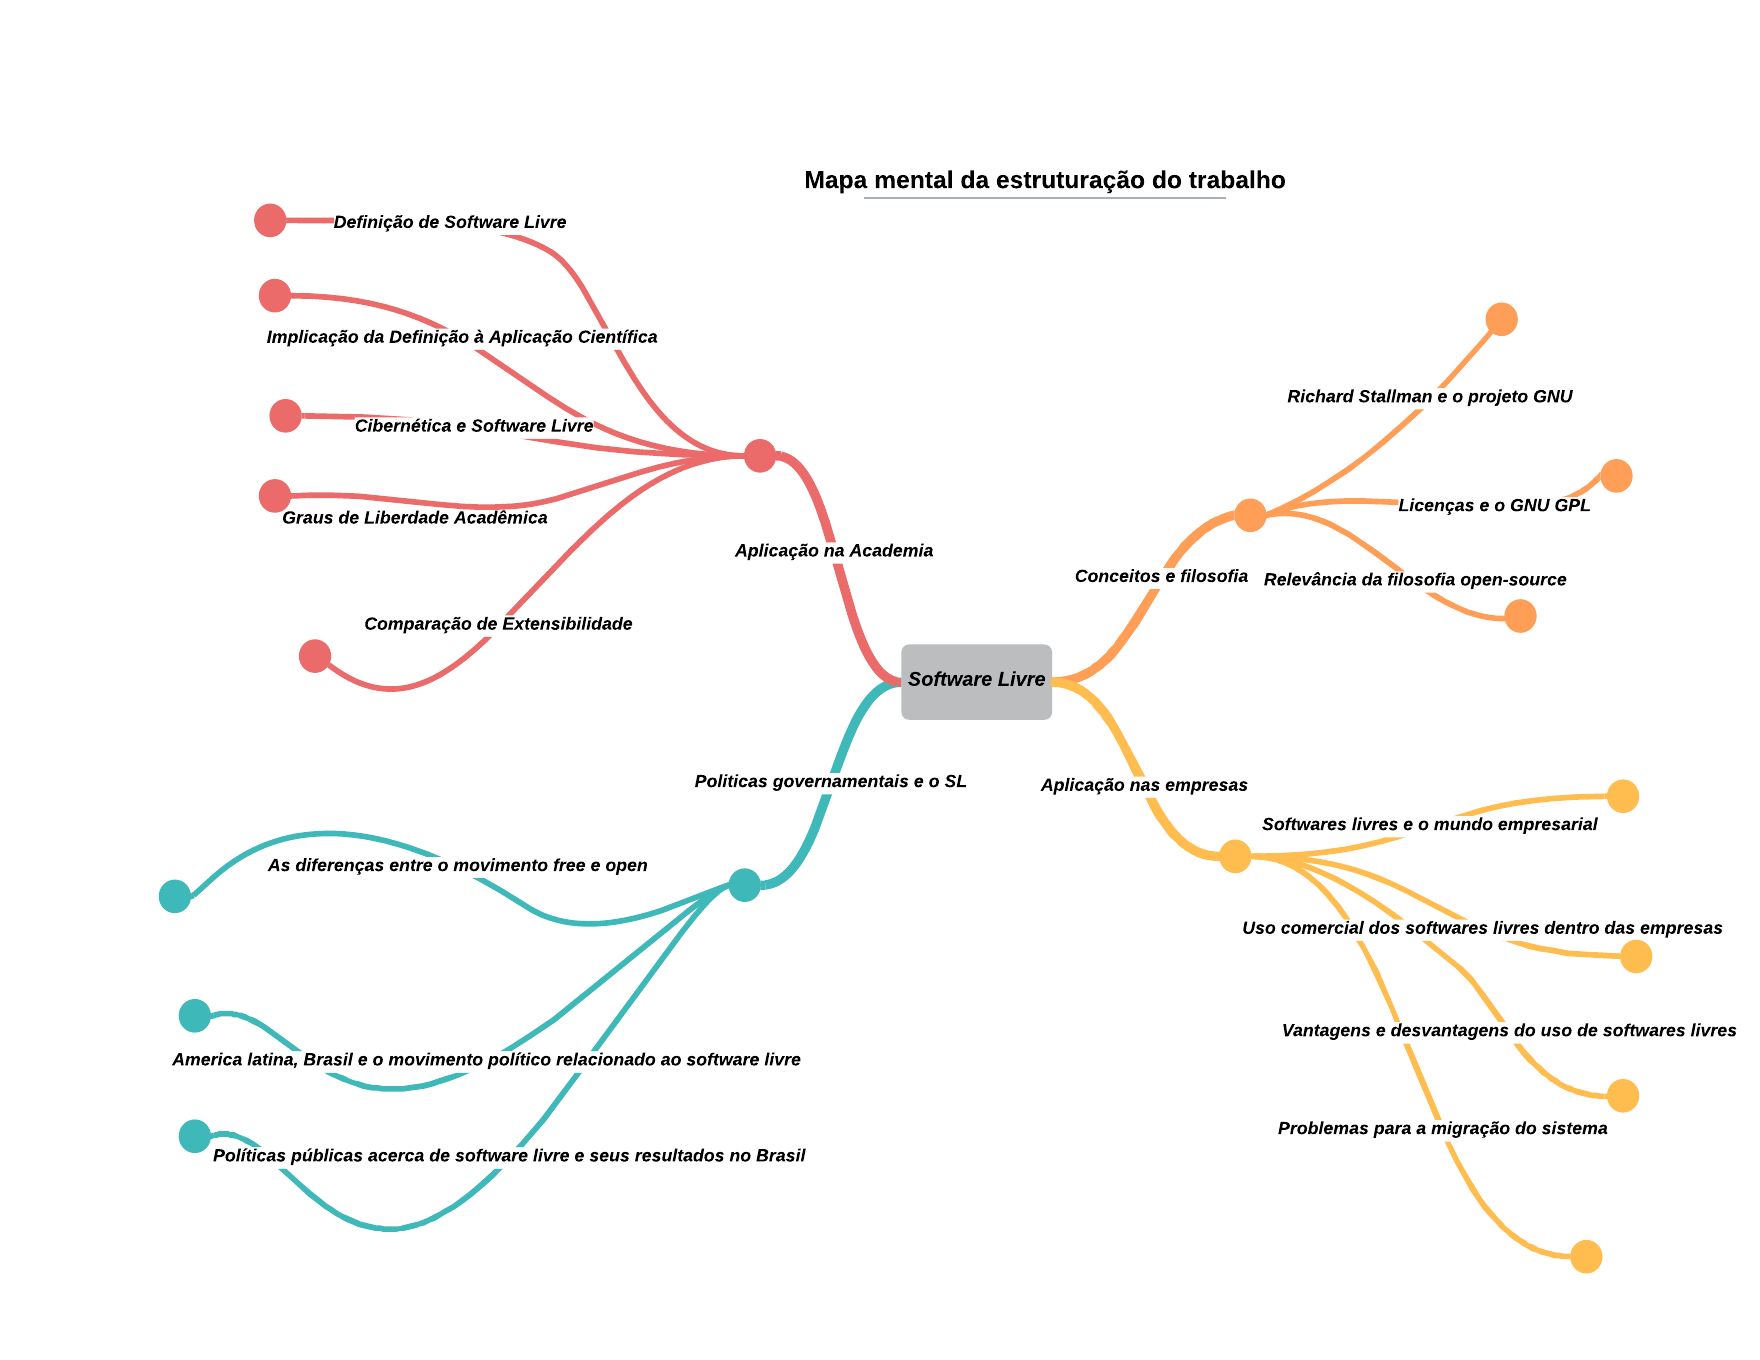
\includegraphics[width=\textwidth]{images/Mapa mental com linhas (1).png}
    \legend{Fonte: os autores}
  \end{center}
\end{figure}

O levantamento de informações acerca o uso de \textit{softwares} livres utilizados nas áreas industrial e empresarial vai se dar por meio de leituras de documentos científicos anteriores que tratam sobre o assunto, além do uso de canais de informação \textit{online} que possuem informações discutidas setor de tecnologia, que informaram alguns dados sobre o uso e funcionalidades dos \textit{softwares} dentro das empresas, além de informarem um pouco sobre o panorama das indústrias e empresas em relação aos \textit{softwares}.

No meio acadêmico, os aspectos os quais são relevantes, ultimamente a qualidade da experiência de se utilizar o software. Devido à abertura dos códigos, bem como ser parte da integração de uma comunidade, a qual, de longe, ultrapassa em quantidade e qualidade a de qualquer empresa específica. E, assim, para um cientista, a experiência de utilizar \textit{softwares} livres traz tanto um senso de irmandade, quanto de profundidade e qualidade para seu trabalho. Pois, nele, aprende com o código, incrementa-o com seu conhecimento e ideias, quanto também, estabelece contato com um novo mundo de programadores-usuários.

Por outro lado, o estado como um agente que faz também uso de novas tecnologias, mas com um propósito, em grande parte, filantrópico, é ilustrado nesse levantamento bibliográfico como um estudo de caso brasileiro. No Brasil, em 2003 foi empregado um decreto presidencial que estabelecia o uso preferencial de software de código aberto que deu início a um desenvolvimento tecnológico pautado na democratização do acesso\cite{torres2018software}.

A Figura \ref{fig:fluxograma} mostra a partir de um fluxograma as ações tomadas pela equipe para a montagem do trabalho.

\begin{figure}[H]
  \begin{center}
    \caption{\label{fig:fluxograma}Fluxograma da metodologia utilizada para o estudo do tema}
    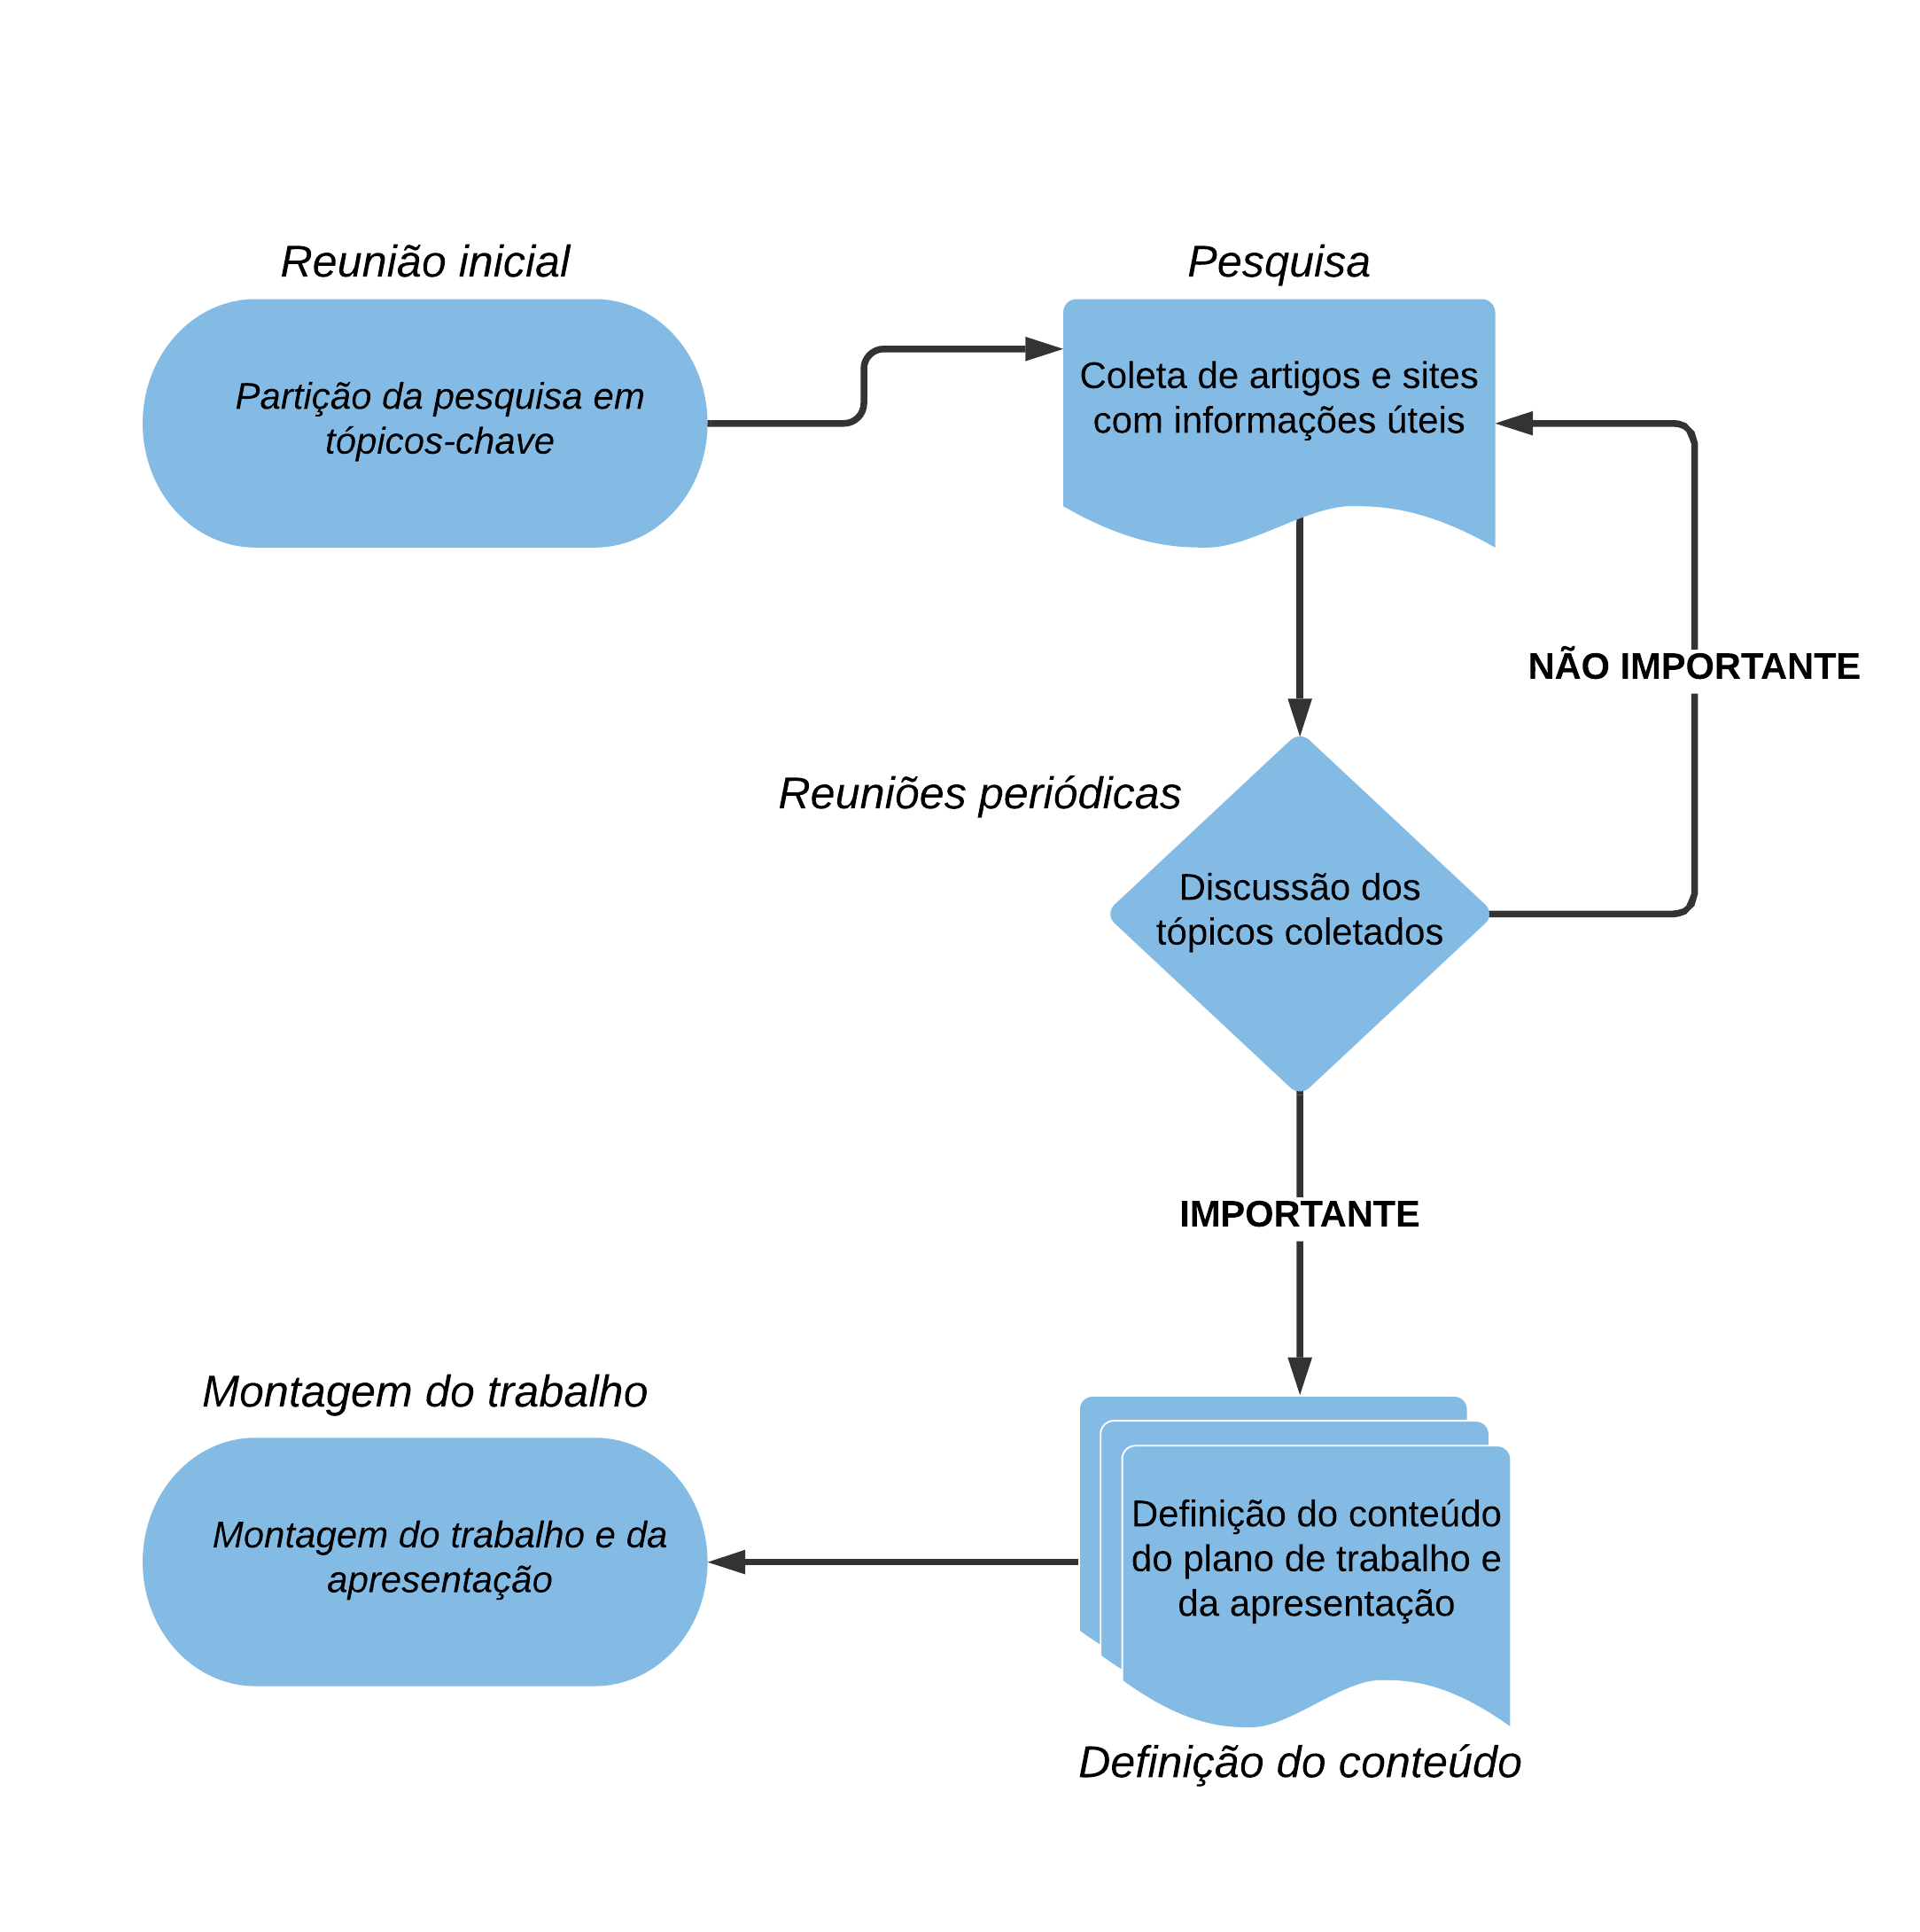
\includegraphics[width=0.9\textwidth,height=\textheight,keepaspectratio]{images/_Fluxograma Plano de Trabalho.png}

    \legend{Fonte: os autores}
  \end{center}
\end{figure}

%%%%%%%%%%%%%%%%%%%%%%%%%%%%%%%%%%%%%%%%%%%
%% COMANDO DE FIGURA
% \begin{figure}[!ht]
%   \centering
%   \caption{\label{fig:frog}Exemplo de figura. A legenda deve vir em cima da figura e %deve conter informações relevantes para a sua compreensão.}
%   \includegraphics[width=\textwidth]{frog.jpg}
%   \caption*{Fonte: creative commons Wikipedia.}
% \end{figure}

%%%%%%%%%%%%%%%%%%%%%%%%%%%%%%%%%%%%%%%%%%%
%% COMANDO DE TABELA
% \begin{table}[!ht]
%   \centering
%   \caption{\label{tab:widgets}Exemplo de tabela. A legenda deve vir em cima da tabela %e explicar seu conteúdo.}
%   \begin{tabular}{l|r}
      %       Item & Quantity \\\hline
      %       Widgets & 42 \\
      %       Gadgets & 13\\
      %       \hline
      %       \multicolumn{2}{l}{Fonte: o autor.}
      %     \end{tabular}
      %       \end{table}

      %%%%%%%%%%%%%%%%%%%%%%%%%%%%%%%%%%%%%%%%%%%%
      %%       COMANDO LISTAGEM

      %       \begin{enumerate}
      %       \item Like this,
      %       \item and like this.
      %       \end{enumerate}
      %       \dots ou itens com bolinhas \dots
      %       \begin{itemize}
      %       \item Like this,
      %       \item and like this.
      %       \end{itemize}

      %%%%%%%%%%%%%%%%%%%%%%%%%%%%%%%%%%%%%%%%%%%%
      %%       Exemplo de descrições.

      %       \begin{description}
      %       \item[Word] Definition
      %       \item[Concept] Explanation
      %       \item[Idea] Text
      %       \end{description}

      %%%%%%%%%%%%%%%%%%%%%
      %%%%%%%%%%%%%%%%%%%%%

\newpage

\section{Resultados}
\subsection{Implicação nas indústrias e empresas}

A partir da pesquisa realizada, foi possível, possível notar o grande impacto que os \textit{softwares} livres já possuem dentro das empresas. O \textit{software} Linux muito utilizado nos servidores de grande e médias empresas e em alguns computadores das mesmas já vem rivalizando diretamente com o Unix e o Windows, \textit{softwares} proprietários que já classificam o crescimento do número de usuários de Linux como uma ameaça para seus modelos de negócios.

Além disso, os \textit{softwares} livres oferecem ótimos benefícios econômicos e estratégicos. Como o não pagamento das licenças por período de tempo ou número de máquinas utilizadoras do \textit{software} e a liberdade tecnológica para poder alterar o \textit{software} utilizado para que ele possa atender as suas necessidades. Além disso, para comunidades grandes o suficiente, como a do Linux, uma atualização constante do \textit{software} tornando-o mais seguro, estável e confiável do que os \textit{softwares} proprietários que tem um tempo de demora maior para resolver vulnerabilidades e lançar novas versões.

Por fim os \textit{softwares} permitiram também um novo mercado para empresas que buscam desenvolver seus serviços baseados no uso de \textit{softwares} livres, sendo um dos principais ramos a prestação de serviços e treinamento de outras empresas que desejam migrar o uso de seus \textit{softwares} de proprietários para livres.

\subsection{Políticas governamentais e o SL}
Os resultados obtidos na pesquisa bibliográfica levantada resultam em uma linha do tempo dos principais impactos práticos no Brasil por ter adotado uma política de fortalecimento ao \textit{Software} Livre em um momento da história em que o acesso a internet começava a se popularizar. Essa iniciativa foi estratégica e coordenada de forma que diferentes setores do governo o adotassem, e empresas públicas estratégicas construíssem meios e ferramentas para essa utilização. Na Figura \ref{fig: label-imagem} pode ser visto a linha do tempo dos principais acontecimentos citados na pesquisa bibliográfica, que marcaram o Software Livre como política pública.


\begin{figure}[H]
  \begin{center}
    \caption{Linha do tempo das políticas públicas, em esfera nacional, que fomentaram o uso de software livre}
    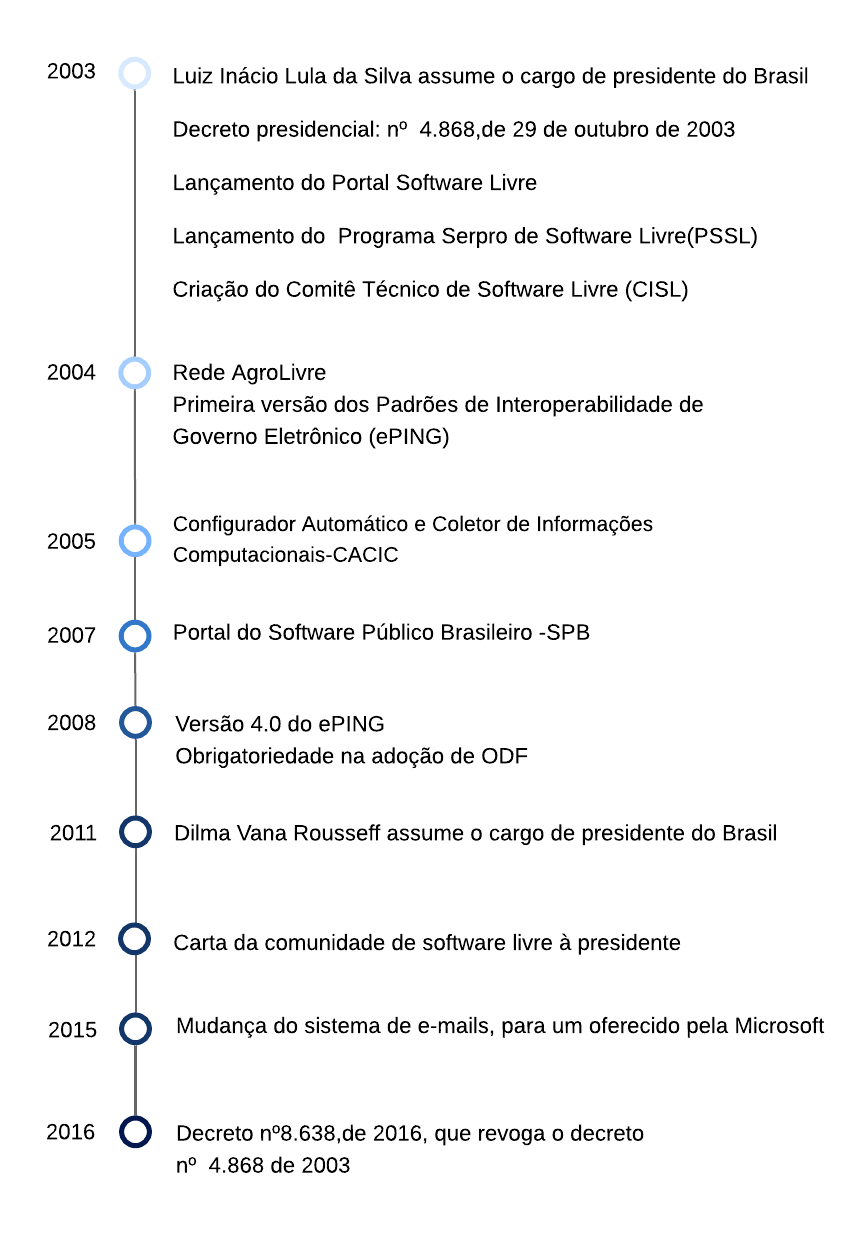
\includegraphics[width=0.9\textwidth,height=\textheight,keepaspectratio]{images/Linha do tempo de um projeto.png}
    \label{fig: label-imagem}

    \legend{Fonte: os autores}
  \end{center}
\end{figure}




A troca de governo foi o começo do fim da iniciativa federal de apoio e adoção do software livre, e o fim demorou até 2016 para acontecer de fato. E com isso finaliza-se o levantamento de como foi a experiência brasileira de adoção do \textit{software} livre em esfera nacional, e além disso, a execução de um projeto percussor de acessibilidade digital e um novo jeito de se fazer uma democracia participativa.

\newpage

\section{Conclusão}

É de suma importância compreender assuntos que tangem a temática de OS. As suas aplicações na nossa nova era de dados são indiscutíveis, e todas as esferas da nossa atual sociedade são afetadas por suas implicações. Neste artigo, algumas delas foram discutidas, em específico a científica, governamental e a empresarial.

O paradigma aberto é normalmente inconcebível quando se tem como base o conhecimento de um livre mercado que opera pela comercialização de propriedades intelectuais. Porém, este conceito introduz na sociedade uma nova dinâmica de interação e colaboração, e que, por evidências claras de constante transformação tecnológica, não corrompe ou afeta a operação do mercado, mas abre espaço para novas possibilidades e modelos de negócio. Ter o direito de acesso completo e livre garantido oferece aos usuários, e por consequência à sociedade, um alicerce robusto no qual todas as tecnologias básicas podem ser desenvolvidas e distribuídas.

Dessa forma algumas empresas começaram a prestar serviços baseados no desenvolvimento e utilização dos \textit{softwares} livres, impulsionando ainda mais seu uso dento do setor empresarial. A capacidade de adaptar o código em conjunto de seus benefícios econômicos gerados pela redução de custos com licenças e renovação frequente dos \textit{hardwares} tornou o uso dos \textit{softwares} livres muito atraente para as empresas, que a partir desse uso puderam ficar mais competitivas. Ademais, no cenário empresarial a evolução do movimento SL tem se tornado cada vez mais uma ameaça para muitas empresas desenvolvedoras de \textit{softwares} proprietários.

As políticas públicas que apoiam o uso e constroem soluções baseadas em software livre são extremamente importantes pois extrapolam a questão técnica e contribuem uma democracia participativa.
No caso do Brasil vemos diversas iniciativas em conjunto que estabeleceram frentes de ações na adoção do software livre, e dentre todos os pontos positivos dessa posição adotada no governo Lula, destacamos: descolonização tecnológica, fortalecimento da mão de obra técnica nacional, incentivo à criação de premissas para o gerenciamento de informações no governo(como a criação do ePING) e ,como se referiu Lula no 10º Fórum Internacional de Software Livre, o avanço no fortalecimento da produção nacional de tecnologia impacta também na autoestima do brasileiro quando se vê como produtor e detentor de um conhecimento tão relevante. Por fim é válido salientar que é uma perda inestimável o fato de que com a troca de gestão foi perdido os investimentos na área e aconteceu a descontinuação de todos os programas começados no governo Lula.
\newpage

\section{Participação autoral}

A participação autoral de cada membro na execução desse trabalho pode ser descrita abaixo:

\begin{itemize}
\item Igor: levantamento de tópicos associados aos principais conceitos e pontos da filosofia OS e de sua história; estudo sistemático de licenças empregadas em códigos abertos; análise da extensão da filosofia a outros segmentos; contribuição para a montagem do relatório.

\item Camila: levantamento, escrita e apresentação dos resultados dos tópicos que fundamentaram as relações das políticas governamentais que trouxeram o software livre para a prática brasileira; colaboração na construção da metodologia; criação do mapa mental da estrutura do trabalho; contribuição da montagem do relatório; participação das reuniões para delimitar e ajustar o trabalho.

\item Pedro: pesquisa em relação aos aspectos do S.L. os quais contrastam com os \textit{Softwares} Proprietários, dentro da esfera acadêmica. Ajuda na formatação do documento, utilizando personalizações de pacotes, e criando comandos para estender os comportamentos de funções do \LaTeX.

\item Alexandre: levantamento de informações relacionadas a aplicação nas empresas; apresentação dos resultados referentes ao uso do \textit{softwares} livres nas empresas; criação do fluxograma executado pela equipe; contribuição para a montagem do relatório; formatação do documento; participação das reuniões que definiram os rumos do trabalho.

\item Henrique: contribuição e discussão relacionadas aos temas; participação das reuniões para delimitar e ajustar o trabalho; organização e formatação textual; criação de imagens apresentadas no trabalho.
\end{itemize}


\clearpage


      %       Nesse formato apresentado aqui em \LaTeX a ordem apresentada abaixo corresponde ao número no texto, ou seja, a primeira referência citada não será de número 1 e sim a primeira a ser colocada na lista abaixo.

      %       \bibliography{bibliografia} pra quem sabe usar arquivos .bib

      %%       If you have bibdatabase file and want bibtex to generate the
      %%       bibitems, please use
      %%
      %%       \bibliographystyle{elsarticle-num}
      %%       \bibliography{<your bibdatabase>}

      %%       else use the following coding to input the bibitems directly in the
      %%       TeX file.


\bibliography{ref.bib}
\bibliographystyle{apalike}
\addcontentsline{toc}{section}{Referências}

\end{document}

%%% Local Variables:
%%% mode: latex
%%% TeX-master: t
%%% End:
